\chapter{Background}\label{chap:background}
\begin{overview}
  In this chapter, background information is presented on the commercial MPC software used. 
  Information regarding the test problems and case studies investigated, are also presented here.
\end{overview}

\section{Commercial MPCs}
The general concepts of MPCs have been discussed in section \ref{sec:mpclit}.
This section gives a more detailed description of two popular commercial MPC packages.
\subsection{Honeywell RMPCT}
Honeywell's MPC controller, RMPCT, forms part of their advanced process control suite, Profit Suite.
A brief overview of the controller and optimizer is given below. 
Attention is given to the controller internals as well as the interface used to build such a controller.
The information presented in this section is taken from \citet{honeywell1}, \citet{honeywell2} and \citet{honeywell3} unless stated otherwise.

\subsubsection{Models}
For the purpose of predictions, process models usually need to be identified first -- typically done via step testing.
\citet{honeywell3} lists the types of models which are supported by the Identifier and elaborates on their specific application.
These model types include;
\begin{itemize}
\item FIR,
\item PEM (the structure of which supports FIR, ARX, ARMA, ARMAX, ARIMA(X), ARARMAX, BJ and OE models) and
\item Laplace domain parametric models.
\end{itemize}
The final model, however, is saved in the Laplace domain.
Discrete models are converted to the {\it s} domain and has a final structure as shown in equation \ref{eq:rmpctmodel}.
\begin{equation}
  \label{eq:rmpctmodel}
  G(s) = \frac{k(b_{n-1}s^{n-1}+ \cdots b_1s+1)e^{-ds}} {s(a_ns^n+a_{n-1}s^{n-1}+ \cdots a_1s+1)}
\end{equation}
The leading {\it s} in the denominator of equation \ref{eq:rmpctmodel} indicates an integrator in any of the sub-processes.

If a third-party model exists, then the model converter in Profit Suite can be used to convert it into a suitable form.
  
\subsubsection{Constraints}
For MVs, the implementation of control constraints are in the form of high/low limits and movement limits.
The high/low limits of MVs are never violated.
Prioritisation and move suppression of MVs are done by means of weighting factors.
The movement load is spread across the MVs as per equation \ref{eq:rmpctmvload},
\begin{equation}
  \label{eq:rmpctmvload}
  \min \sum_j \Delta u_j^2 \times weight_j^2
\end{equation}
where $j$ is the index of the MV.

CV control constraints are also specified as high/low limits.
In the event of negative degrees of freedom, constraints are prioritised by means of a give-up factor called the engineering unit (EU) give up.
Similar to equation \ref{eq:rmpctmvload} the cumulative weighted error on the CVs are minimised as per equation \ref{eq:rmpctcverror} with the $weight$ defined as shown and where $i$ is the CV index.
\begin{align}
  \label{eq:rmpctcverror}
  \min \sum_i weight_i^2 \times error_i^2 \\
  weight = \frac{1}{(\text{CV scaling factor})_i\sqrt{(\text{EU give up})_i}} \notag
\end{align}

The optimisation constraints are defined as being a specified amount within the high/low control limits.
These limits are not used for control.
For the constraining of dynamic response, funnels are implemented.
Predefined funnel types can be chosen from;
\begin{itemize}
\item Type 0, which is an automatically generated funnel,
\item Type 1, defined as a third of the Type 0 funnel pinched using the feedback performance ratio (FPR), and
\item Type 2, which is like Type 1 but pinched with the decouple ratio (Type 2 is therefore FPR independent).
\end{itemize}
Figure \ref{fig:rmpctfunnel} illustrates the concept of pinching for the RMPCT funnels.
The definitions of the FPR and the decouple ratio are contained in \citet{honeywell1} but omitted from this dissertation.
\begin{figure}[htbp]
  \centering
  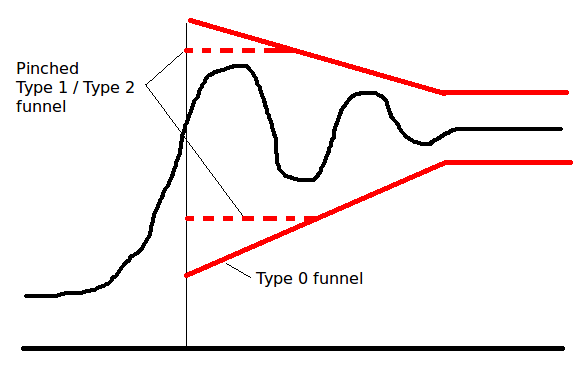
\includegraphics[width=8cm]{rmpct_funnel}
  \caption[RMPCT funnel implementation]{RMPCT funnel implementation showing pinched funnels with dashed lines.}
  \label{fig:rmpctfunnel}
\end{figure}

\subsubsection{Interface}
Profit Design Studio is used for model identification.
From this interface the process model can be extracted.
All the constraints (as discussed in the preceding section) can be added using this interface, where after the controller is built for on-line use.

The operator interface, Profit Suite Operator Station, allows for constraint changes during plant operation.
As far as feasibility of constraints are concerned, these constraints are only checked to be within the Engineering limits (an additional constraint present in this interface).
A gain matrix (the steady-state model) can easily be obtained from this interface.

%screenshots?

\subsection{AspenTech DMCPlus}
Aspen Technologies' MPC controller, DMCPlus, forms part of their advanced process control suite, aspenONE.
The overview presented in this section is taken from \citet{aspentech1} unless stated otherwise.

\subsubsection{Models}
Model identification is done with DMCplus Model or with SmartStep which enables model identification whilst still maintaining control of a plant.
Models are stored as FIR models and conversion to and from other model types are not supported.
Extracting a steady-state gain matrix is however possible.

\subsubsection{Constraints}
As with RMPCT, constraints on the CVs and MVs are specified as high/low limits.
Equal concern errors (ECEs) are used to calculate the optimal move plan and emphasise the relative importance of CVs.

For constraint handling, rank groups are used.
Constraints are ranked and lower rank constraints are considered ``hard'' whereas higher ranking constraints are relaxed until steady-state feasibility is achieved.
%% EXPAND

\subsubsection{Interface}
%% EXPAND

\section{Case studies}

\section{Test problems}

% Local Variables:
% TeX-master: "AHC_thesis"
% End: